\section{Introduction}\label{sec:Charmonia_Theory}

This section provides an introduction to the physics of charmonia in hadronic and heavy-ion collisions. The basic properties of charmonium states are detailed in \sect{sec:Charmonia_Theory_CharmoniumStates}, followed by a brief description of different models of charmonium hadroproduction in \sect{sec:Charmonia_Theory_HadronicProduction}. A short overview of some nuclear matter effects that can impact the measurement of charmonium production in heavy-ion collisions is presented in \sect{sec:Charmonia_Theory_HeavyIon}, as well as the current understanding of their role in the past measurements.

\subsection{Spectrum of charmonium states}\label{sec:Charmonia_Theory_CharmoniumStates}

Charmonia are bound states of a charm quark and anti-quark. They are part of the family of quarkonium mesons, briefly introduced in \sect{sec:Physics_HI_Probes_Quarkonium}. The first observation of a charmonium state was published in 1974, by the collaborations lead by Burton Richter at SLAC~\cite{JPsiDiscovery_2} and Sam Ting at BNL~\cite{JPsiDiscovery}. Both experiments found a narrow resonance in the \elel and \mumu decay channels with an invariant mass of $m \approx 3.1$~\GeVcc, which was named J by Sam Ting and $\psi$ by Burton Richter, thus later referred as the \JPsi meson.

Following a non-relativistic approach, by solving the Schr{\"o}dinger equation using a \ccbar potential model as mentioned in \sect{sec:Physics_HI_Probes_Quarkonium}, the charmonium states can be classified according to the total spin $S$, orbital angular momentum $L$ and total angular momentum $J$ of the \ccbar system.  Depending on the spin of the \ccbar pair, charmonia can either be singlet ($S = 0$) or triplet ($S = 1$). The charmonium states are typically labelled using the notation $n^{2S+1}L_{J}$, where $n$ is the principal quantum number. By convention, the charmonium states with values $L = 0, 1, 2 ...$ are denoted as {S, P, D ...}. In this notation, the \JPsi meson ($n=1, S=1, J=1$) represents the S-wave ground state $1^{3}\text{S}_{1}$, while the \PsiP meson ($n=2, S=1, J=1$) corresponds to its first excited state $2^{3}\text{S}_{1}$. The mass of charmonium states increases with $n$, being larger for higher excited states. \tab{tab:CharmoniaMassWidth} summarises the mass and width of some charmonium states.

\begin{table}[htb!]
 \centering
 \begin{tabular}{| c | c | c | c |}
  \hline
  Charmonium state & $n^{2S+1}L_{J}$ & Width [\MeVcc] & Mass [\MeVcc] \\ \hline
  $\eta_{\cPqc}(1\text{S})$ & $1^{1}\text{S}_{0}$ & $32.1 \pm 0.9$ & $2983.9 \pm 0.5$ \\ \hline
  \JPsi & $1^{3}\text{S}_{1}$ & $0.0929 \pm 0.0028$ & $3096.900 \pm 0.006$\\ \hline
  $h_{\cPqc}$ & $1^{1}\text{P}_{1}$ & $0.70 \pm 0.36$ & $3525.38 \pm 0.11$ \\ \hline
  $\chi_{{\cPqc}0}$ & $1^{3}\text{P}_{0}$ & $10.5 \pm 0.8$ & $3414.71 \pm 0.30$ \\ \hline
  $\chi_{{\cPqc}1}$ & $1^{3}\text{P}_{1}$ & $0.88 \pm 0.05$ & $3510.67 \pm 0.05$ \\ \hline
  $\chi_{{\cPqc}2}$ & $1^{3}\text{P}_{2}$ & $2.00 \pm 0.11$ & $3556.17 \pm 0.07$ \\ \hline
  $\eta_{\cPqc}(2\text{S})$ & $2^{1}\text{S}_{0}$ & $11.3^{+3.2}_{-2.9}$ & $3637.6 \pm 1.2$ \\ \hline
  \PsiP & $2^{3}S_{1}$ & $0.294 \pm 0.008$ & $3686.097 \pm 0.010$ \\
  \hline
 \end{tabular}
 \caption{The width and mass of charmonium states below the $\D\bar{\D}$-meson pair mass. Information taken from Ref.~\cite{PDG}.}
 \label{tab:CharmoniaMassWidth}
\end{table}

The branching ratios for charmonium decays depend on the mass of the bound state. On the one hand, charmonium states with masses above two times the \D-meson mass ($m_{\D}$), that is 3.73~\GeVcc, preferentially decays to open-charm hadrons (i.e. with non-zero charm quantum numbers, such as \D mesons or charmed baryons), favoured by the Okuba-Zweig-Iizuka (OZI) rule~\cite{OZI_1,OZI_2,OZI_3}. On the other hand, charmonium states with masses below $2m_{\D}$, decays radiatively (e.g. $\chi_{\cPqc} \rightarrow \JPsi + \gamma$) or hadronically (e.g. $\PsiP \rightarrow \JPsi + 2\pi$) to lower mass charmonium states or light hadrons, and also electromagnetically to lepton pairs. As a result, charmonium states below the $\D\bar{\D}$ threshold appear as mass peaks in the dilepton invariant mass distribution, while those above do not. The different charmonium decays to lower mass charmonia are shown in \fig{fig:CharmoniaDecay} and the main branching ratios for decays of \JPsi and \PsiP mesons are presented in \tab{tab:CharmoniaSWave}.

\begin{figure}[htb!]
 \centering
 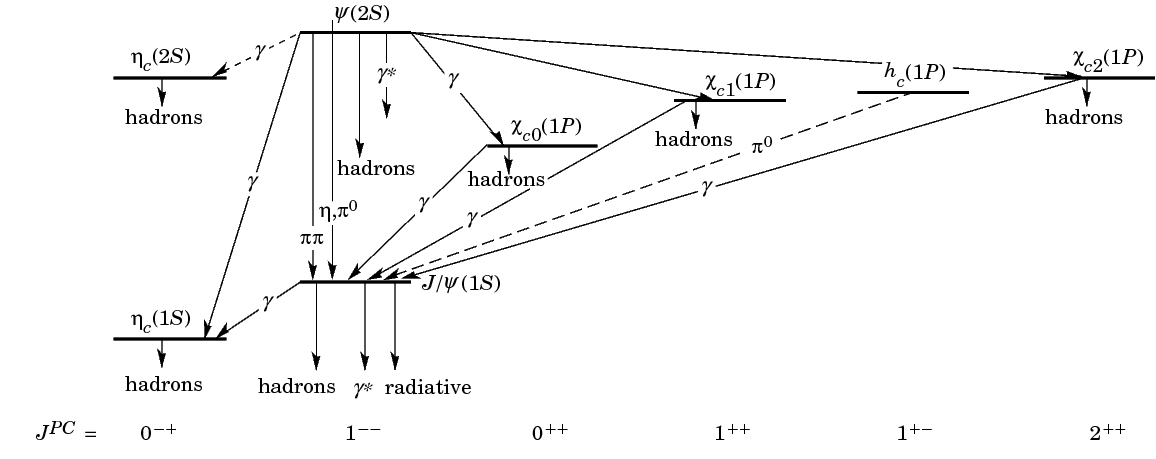
\includegraphics[width=1.0\textwidth]{Figures/Charmonia/Theory/States/CharmoniaDecays.png}
 \caption{Illustration of the different charmonium decays to lower mass charmonium states. The dashed (solid) lines represent radiative (hadronic) decays. Figure taken from Ref.~\cite{CharmoniumDecays}.}
 \label{fig:CharmoniaDecay}
\end{figure}

\begin{table}[htb!]
 \centering
 \begin{tabular}{ | c | c  c  c |}
  \hline
  \multirow{2}{*}{Charmonium} & \multicolumn{3}{c|}{Branching ratio [\%]} \\
   & \mumu & \elel & hadrons \\ \hline
  \JPsi & $5.961 \pm 0.033$ & $5.971 \pm 0.032$ & $87.7 \pm 0.5$ \\ \hline
  \PsiP & $0.80 \pm 0.06$ & $0.793 \pm 0.017$ & $97.86 \pm 0.13$ \\
  \hline
 \end{tabular}
 \caption{Branching ratios for decays of \JPsi and \PsiP mesons. Information taken from Ref.~\cite{PDG}.}
 \label{tab:CharmoniaSWave}
\end{table}


\subsection{Hadroproduction of charmonia}\label{sec:Charmonia_Theory_HadronicProduction}

Charmonia can be produced from various sources including: the initial hard scattering (direct), decays of higher mass charmonium states (feed-down), or weak decays of hadrons containing bottom quarks. Directly produced charmonium states or those from feed-down contributions are known as \textit{prompt}, while charmonium states from b-hadron decays are called \textit{nonprompt}. A brief introduction to some of the models used to describe the production of charmonia in hadron collisions are presented in the following sub-sections.

\subsubsection{Colour singlet model}\label{sec:Charmonia_Theory_HadronicProduction_CSM}

The Colour Singlet Model (CSM) was first proposed in 1975 by Martin Einhorn and Stephen Ellis~\cite{CSM_1,CSM_3}, to describe the hadroproduction of $\eta_{\cPqc}$ mesons. It assumes that the quantum numbers of the \ccbar pairs do not change between their production and subsequent hadronisation into charmonia. As a consequence, the \ccbar pair has the same angular momentum, spin and colour charge as the charmonium state it eventually forms and since all hadrons are colour singlets, the CSM requires the \ccbar pair to be produced in a colour singlet state. The model also considers charmonia as non-relativistic bound states, neglecting the relative momentum of the charm quarks inside the charmonium~\cite{CSM_2}. Under these conditions, the probability that a colour-singlet \ccbar pair becomes a charmonium state is proportional to the square of the \ccbar wave function and its derivatives, evaluated at the origin in position space. The inclusive cross section of the production of a S-wave charmonium state $\Psi$ in collisions of hadrons $h_{A}$ and $h_{B}$, is given in the CSM by~\cite{Quarkonium_Overview}:

\begin{equation}
 \sigma^{\text{CSM}}\left[h_{A}h_{B} \rightarrow \Psi + X\right] = {{\sigma}\left[h_{A}h_{B} \rightarrow \ccbar_{\left[1\right]}+ X\right]}{\cdot}{\abs{\psi_{\ccbar}\left(0\right)}^{2}}
\end{equation}

where ${\sigma}\left[h_{A}h_{B} \rightarrow \ccbar_{\left[1\right]}+ X\right]$ is the hadroproduction cross section of a colour-singlet \ccbar pair, and $\psi_{\ccbar}$ is the corresponding \ccbar wave function. The main advantage of the CSM is that it becomes fully predictive once the magnitudes of the \ccbar wave functions are fixed, since it does not contain any other free parameters. The $\abs{\psi_{\ccbar}\left(0\right)}^{2}$ can be determined from experimental measurements of charmonium decay widths or using potential models of the \ccbar system~\cite{Lansberg_Quarkonium}.

The CSM has been able to describe the bulk production of charmonia at RHIC~\cite{Lansberg_RHIC}, but it significantly underestimates the \pt-differential cross section of prompt charmonia measured in \Runppbar collisions at Tevatron~\cite{Charmonium_Tevatron}. Moreover, the model suffers from infrared divergences when extending the calculations to charmonium states with nonzero orbital angular momentum (e.g. $\chi_{\cPqc}$ meson)~\cite{Quarkonium_Overview_2}. However, the inclusion of NLO and NNLO corrections in $\alpha_{s}$ improves the agreement with the experimental results~\cite{Lansberg_Quarkonium}.

\subsubsection{Colour evaporation model}\label{sec:Charmonia_Theory_HadronicProduction_CEM}

The Colour Evaporation Model (CEM) is an alternative model of charmonium production, introduced by Harald Fritz~\cite{CEM_1} and Francis Halzen~\cite{CEM_2} in 1977. Contrary to the CSM, the CEM allows the quantum states of the \ccbar pair to change during its evolution. In the CEM, a charmonium state can be produced from any \ccbar pair with an invariant mass between the threshold to create a charm-quark pair $2m_{\cPqc}$ and the one to produce the lightest pair of open-charm hadrons $2m_{\D}$ (i.e. $\D$-meson pair). The CEM does not impose any constrains on the colour charge of the \ccbar pair in order to form a charmonium state, and instead assumes that the colour state of the \ccbar pair is neutralised via soft gluon interactions with the collision-induced medium after its production (this process is called colour evaporation). In addition, the interaction with the medium is assumed to randomise the spin and angular-momentum states of the \ccbar pairs, making the CEM insensitive to the polarization of charmonia. The probability that \ccbar pairs, with an invariant mass below $2m_{\D}$, hadronise into a charmonium state is represented by a fraction $F_{\psi}$, which is assumed to be constant and universal (i.e. does not depend on the \ccbar kinematics or the hard process)~\cite{Quarkonium_Overview_2}. In the CEM, the hadronic cross section for the production of a charmonium state $\psi$ is defined as:

\begin{equation}
 \sigma^{\text{CEM}}\left[h_{A}h_{B} \rightarrow \psi + X\right] = F_{\psi}{\int_{2m_{\cPqc}}^{2m_{\D}}{\dd{m}_{\ccbar}}}\frac{\dd{{\sigma}}\left[h_{A}h_{B} \rightarrow \ccbar+ X\right]}{\dd{m}_{\ccbar}}
\end{equation}

where $m_{\ccbar}$ is the invariant mass of the \ccbar pair, and ${\sigma}\left[h_{A}h_{B} \rightarrow \ccbar+ X\right]$ is the hadronic cross section of the production of \ccbar pairs, averaged over all spin, angular-momentum and colour-charge states. The only free parameters of the CEM are the fractions $F_{\Psi}$, which are constrained with experimental data. The description of the \pt distribution of charmonia requires to consider contributions from at least NLO, which includes \ccbar-pair production associated with gluons or light (anti-)quarks~\cite{CEM_NLO}.

The CEM has been successful at describing the overall hadronic production of charmonium states~\cite{CEM_Experiment}, but it fails to explain the differences observed between the hadroproduction and photoproduction measurements~\cite{Quarkonium_Overview_2}, and the relative production rates between the $\chi_{c1}$ and $\chi_{c2}$ states measured at Tevatron~\cite{CEM_Chic_Tevatron} and LHC~\cite{CEM_Chic_LHC}. Recent developments have lead to an improved version of the CEM~\cite{ICEM}, which attempts to describe the \pt-dependence of charmonium polarization by sorting the states based on their spin.

\subsubsection{Nonrelativistic QCD}\label{sec:Charmonia_Theory_HadronicProduction_NRQCD}

NonRelativistic QCD (NRQCD) is an effective quantum field theory formulated in 1992 by Geoffrey Bodwin, Eric Braaten and Peter Lepage~\cite{NRQCD}, in an attempt to cure the infrared divergences present in the CSM calculations of P-wave charmonium states. The production and decay of charmonia involves large momentum scales, such as the charm-quark mass ($m_{\cPqc} = 1.29~\GeVcc$) or the parton momentum scales during the hard scattering, which are much larger than $\Lambda_{\text{QCD}} \approx \SI{255}{\MeV}$. As a result, the $\alpha_{s}$ value associated to the formation of \ccbar pairs are small enough ($\alpha_{s}(m_{\cPqc}) \approx 0.25$) for perturbation theory to be applied. However, the hadronisation of \ccbar pairs to charmonium states involves low-momentum processes which are inherently nonperturbative~\cite{Quarkonium_Overview_2}.

The NRQCD formalism makes use of perturbative calculation techniques by separating the high-momentum (short-distance) perturbative effects (\ccbar-pair production) from the low-momentum (long-distance)  nonperturbative effects (charmonium formation), in a process called factorisation. The NRQCD factorisation approach matches the derivations from full QCD at momentum scales less than $m_{\cPqc}v_{\cPqc}$, where $v_{\cPqc}$ is the mean velocity of bound charm quarks in the charmonium CM frame. Since $v_{\cPqc}$ is low for charmonia ($v^{2}_{\cPqc} \approx 0.3$), the NRQCD calculations are simplified by applying nonrelativistic approximations~\cite{Quarkonium_Overview_2}. The inclusive cross section for the production of a charmonium state $\psi$ with $\pt \geq m_{\cPqc}$, from collisions of hadrons $h_{A}$ and $h_{B}$, is determined in NRQCD by:

\begin{equation}
 \sigma^{\text{NRQCD}}\left[h_{A}h_{B} \rightarrow \psi + X\right] = \sum\limits_{n}{{\sigma}\left[h_{A}h_{B} \rightarrow \ccbar_{\left[n\right]}+ X\right]\left(\mu_{\Lambda}\right)}{\cdot}{\left\langle{\euscr{O}_{n}^{\psi}}\right\rangle}
 \label{eq:NRQCD}
\end{equation}

where $\mu_{\Lambda}$ is an ultraviolet cutoff parameter. The nonperturbative coefficient $\left\langle{\euscr{O}_{n}^{\psi}}\right\rangle$, called Long-Distance Matrix Element (LDME), is the vacuum expectation value of the NRQCD four-fermion operator $\mathscr{O}^{\Psi}_{n}$ and defines the probability for a \ccbar pair in a given quantum state $n$ to evolve into a charmonium state $\psi$. The LDMEs contain the nonperturbative components related to the hadronisation of the \ccbar pairs into charmonia. These matrix elements are process independent and can be constrained by fitting experimental data~\cite{Quarkonium_Overview_2}. Moreover, the perturbative coefficient ${\sigma}\left[h_{A}h_{B} \rightarrow \ccbar_{\left[n\right]}+ X\right]$ represents the hadronic cross section for the production of \ccbar pairs in a quantum state $n$ and can be computed using pQCD. One important remark of NRQCD is that the \ccbar pairs are not required to be produced with the same spin, angular momentum and colour charge as the charmonium states that they eventually hadronise to. As a consequence, the \ccbar pairs can either be produced in a colour-singlet or colour-octet state~\cite{Quarkonium_Overview_2}. Examples of Feynman diagrams involved in the  production of \JPsi mesons from colour-singlet or colour-octet \ccbar pairs are shown in \fig{fig:CharmoniaProd}.

\begin{figure}[htb!]
 \centering
 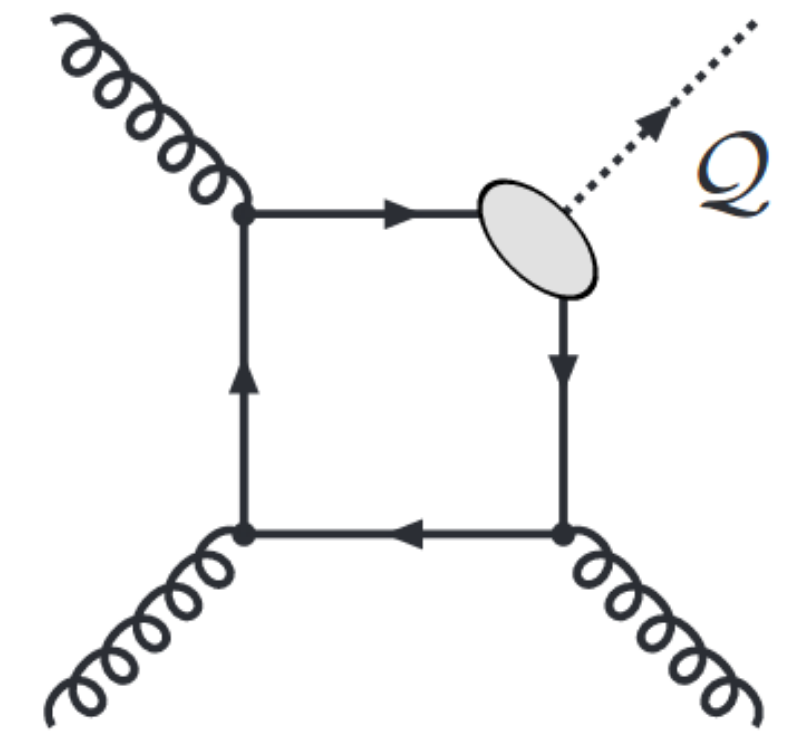
\includegraphics[width=0.3\textwidth]{Figures/Charmonia/Theory/Production/Quarkonia_LO_ColourSinglet.png} \hspace{50pt}
 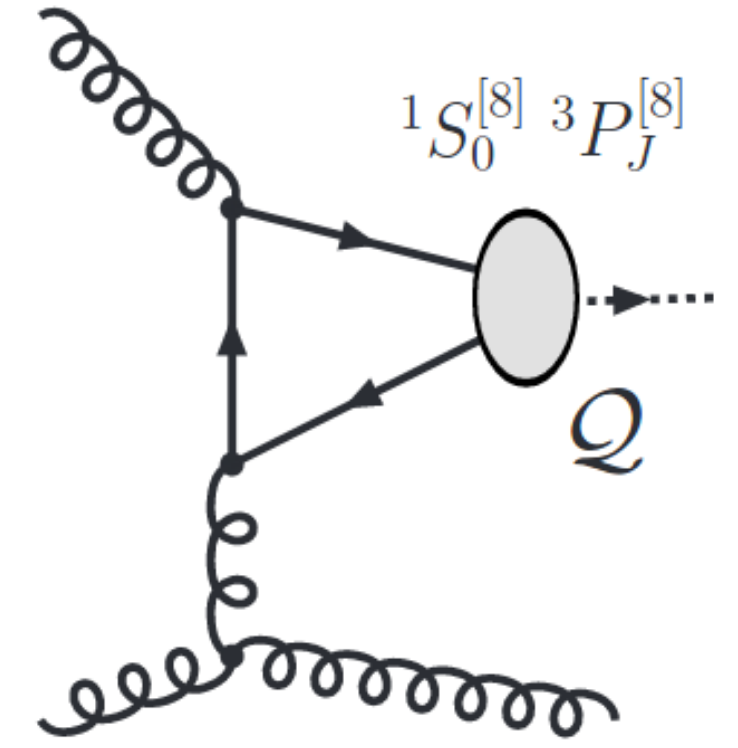
\includegraphics[width=0.3\textwidth]{Figures/Charmonia/Theory/Production/Quarkonia_LO_ColourOctet.png}
 \caption{Illustration of a colour-singlet (left) and colour-octet (right) Feynman diagram, at leading order ($\alpha_{s}^{3}$), that contribute to the production of quarkonium states. Diagrams taken from Ref.~\cite{CharmoniumColourDiagrams}. }
 \label{fig:CharmoniaProd}
\end{figure}

In practice, the sum over the quantum states shown in \eq{eq:NRQCD} is expanded in terms of $v_{\cPqc}$ and $\alpha_{s}$. The infinite number of independent matrix elements is then reduced to a finite set of LDMEs by truncating the sum up to a given order in $v_{\cPqc}$ and making use of spin symmetry relations between charmonium states. At leading order in $v_{\cPqc}$, the S-wave charmonium multiplets (e.g. \JPsi and $\eta_{\cPqc}$) are described by four LDMEs (one colour singlet and three colour octets)~\cite{Quarkonium_Overview_2}, and the CSM can then be recovered by keeping only the colour-singlet term.

NRQCD has been very successful at describing the hadroproduction yield of charmonia at Tevatron, RHIC and LHC~\cite{NRQCD_ATLAS,NRQCD_LHCb,NRQCD_EXPYIELD,NRQCD_EXPYIELD_2}. However, it fails to describe the \JPsi-meson polarization results in hadronic collisions at the Tevatron~\cite{NRQCD_POLFAIL_2} and LHC~\cite{NRQCD_POLFAIL}. In addition, recent measurements of prompt \JPsi mesons in jets produced in \Runpp collisions at $\sqrts = \SI{5.02}{\TeV}$~\cite{NRQCD_JETFAIL_2,NRQCD_JETFAIL}, have shown significant deviations from the NRQCD calculations derived with the \PYTHIA event generator.

\subsubsection{Charmonium production from b-hadron decays}\label{sec:Charmonia_Theory_HadronicProduction_Nonprompt}

The decay of b hadrons constitute an important contribution to the production of charmonia. Bottom quarks are copiously produced at the LHC, mainly through the gluon fusion process ($g + g \rightarrow \cPqb + \cPaqb + X$). They hadronise to \B mesons and b baryons (e.g. $\Lambda_{\cPqb}$ and $\Sigma_{\cPqb}$ baryons), which can then decay weakly into charmonia as shown in \fig{dia:BMesonDecay}. The branching ratios for inclusive decays of b hadrons ($h_{\cPqb}$) into charmonia, $BR(h_{\cPqb} \rightarrow \psi + X)$, have been determined by combining the measurements of b baryons and \B mesons, performed at LHC, LEP, Tevatron and Sp{\PAp}S, and are listed in \tab{tab:BHadronBRCharmonia}.

\begin{figure}[htb!]
 \centering
 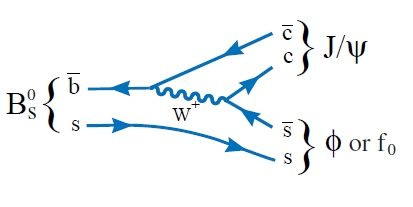
\includegraphics[width=0.6\textwidth]{Figures/Charmonia/Theory/Production/bs_jpsiphi.jpg}
 \caption{Feynman diagram of a $B^{0}_{\cPqs}$ decay to \JPsi meson. Diagram taken from Ref.~\cite{BMesonDecayDiagram}. }
 \label{dia:BMesonDecay}
\end{figure}

\begin{table}[htb!]
 \centering
 \begin{tabular}{| c | c |}
  \hline
  Charmonium state & Branching ratio [\%] \\ \hline
  $\eta_{\cPqc}(1\text{S})$ & $4.5 \pm 1.9$ \\ \hline
  \JPsi & $1.16 \pm 0.10$ \\ \hline
  $\chi_{{\cPqc}0}$ & $1.5 \pm 0.6$ \\ \hline
  $\chi_{{\cPqc}1}$ & $1.4 \pm 0.4$ \\ \hline
  $\chi_{{\cPqc}2}$ & $0.62 \pm 0.29$ \\ \hline
  \PsiP & $0.286 \pm 0.028$ \\
  \hline
 \end{tabular}
 \caption{Branching ratios for inclusive charmonium decays of b-hadron mixtures ($B^{\pm}/B^{0}/B^{0}_{\cPqs}/$b-baryon) determined from measurements at LHC, LEP, Tevatron and Sp{\PAp}S. Information taken from Ref.~\cite{PDG}.}
 \label{tab:BHadronBRCharmonia}
\end{table}

The inclusive cross section of charmonium production from b-hadron decays in \Runpp collisions is described by:

\begin{equation}
 \sigma\left[\pp \rightarrow \cPqb + X \rightarrow \psi + X'\right] = \sum\limits_{j=\text{b hadrons}}\sigma\left[\pp \rightarrow \cPqb + X\right] \otimes D\left(\cPqb \rightarrow h_{\cPqb}^{j}\right) \cdot BR(h_{\cPqb}^{j} \rightarrow \psi + X)
\end{equation}

where $\sigma[\pp \rightarrow \cPqb + X]$ is the total production cross section of bottom quarks in \Runpp collisions and $D(\cPqb \rightarrow h_{\cPqb}^{j})$ is a fragmentation function (FF), which describes the probability that a bottom quark hadronises into a b hadron $h_{\cPqb}^{j}$ with a fraction $z$ of its momentum ($p_{h_{\cPqb}} = z \cdot p_{\cPqb}$). The FFs are considered universal and can be extracted by fitting experimental data. The bottom-quark fragmentation fractions for different b hadrons have been measured at LEP and Tevatron, and the results are shown in \tab{tab:FragmentationBHadrons}.

\begin{table}[htb!]
 \centering
 \begin{tabular}{| c | c  c |}
  \hline
  \multirow{2}{*}{b hadron} & \multicolumn{2}{c|}{Fragmentation fraction [\%]} \\ 
   & $\Z\to\cPqb\cPaqb$ & $\ppbar\to\cPqb\cPaqb + X$ \\ \hline
  $B^{+}$ & $41.5 \pm 0.8$ & $32.4 \pm 2.1$ \\ \hline
  $B^{0}$ & $41.5 \pm 0.8$ & $32.4 \pm 2.1$ \\ \hline
  $B^{0}_{\cPqs}$ & $8.8 \pm 1.3$  & $10.1 \pm 1.5$ \\ \hline
  b baryons  & $8.9 \pm 1.2$  & $21.8 \pm 4.7$ \\
  \hline
 \end{tabular}
 \caption{Fragmentation fractions of bottom quarks into b hadrons measured at Tevatron in \Runppbar collisions at $\sqrts = \SI{1.96}{\TeV}$ and at LEP in $\Z\to\cPqb\cPaqb$ decays. Information taken from Ref.~\cite{PDG}.}
 \label{tab:FragmentationBHadrons}
\end{table}

\subsection{Charmonia in heavy-ion collisions}\label{sec:Charmonia_Theory_HeavyIon}

The observed yields of charmonia are modified in heavy-ion collisions by an interplay of different effects that can take place in the initial or final state of the collision. The effects that originate from the nuclear environment are often called cold nuclear matter (CNM) effects, while those that are caused by the hot and dense medium formed in the collision, the QGP, are known as hot nuclear matter (HNM) effects.

\subsubsection{Cold nuclear matter effects}\label{sec:Charmonia_Theory_HeavyIon_ColdNuclearMatter}

Understanding the impact of the cold nuclear matter effects is crucial to be able to characterise the hot medium produced in heavy-ion collisions. The charmonium production can be affected by several CNM effects, such as nuclear absorption, gluon shadowing, energy loss and Cronin effect.

\paragraph{Nuclear absorption.} After the \ccbar pairs are formed, they will then travel across the nucleus. While crossing the nuclear medium, the \ccbar pair may scatters with the target nucleons. After successive interactions, the \ccbar pair can end up breaking up and the charm quarks then hadronise into open-charm mesons. This process is known as nuclear absorption. The probability that the \ccbar pair survives the nuclear interactions is determined using a Glauber model approach, given by~\cite{Quarkonium_Overview}:

\begin{equation}
 S_{\text{abs}} = \int{\ddd{b}}\int{\dd{z}} \cdot \rho_{A}\left(b,z\right) \cdot \exp\left[-\int^{\inf}_{z}{\dd{z'}} \cdot \rho_{A}\left(b,z'\right) \cdot \sigma_{\text{abs}}\left(z'-z\right)\right]
\end{equation}

where $b$ is the impact parameter of the collision, $\rho_{A}$ is the density profile of the nucleus, $z$ is the position of the \ccbar pair production vertex along the beam direction, and $\sigma_{\text{abs}}$ is an effective cross section used to characterise the nuclear absorption.

To determine the impact of the nuclear absorption on the production of charmonia, it is useful to compare the collision time ($\tau_{\text{coll}}$) to the typical time needed to form a charmonium state ($\tau_{\psi}$). The collision time is defined as the time it takes for two Lorentz-contracted nuclei to cross, given by $\tau_{\text{coll}} = 2R\big/\gamma_{\text{CM}}$~\cite{CollisionTime}, where $\gamma_{\text{CM}} = \sqrtsnn\big/m_{p}$ is the beam Lorentz $\gamma$ factor in the CM frame, $m_{p} = 938$~\MeVcc is the proton mass and $R$ is the radius of the nuclei ($\approx 6.62$~fm for a \Pb nucleus~\cite{PbRadius}). Considering \RunPbPb collisions at $\sqrtsnn = \SI{5.02}{\TeV}$, the collision time is less than 0.003~\fmc which is much smaller than the formation time of charmonia ($\tau_{\psi} \sim 0.4$~\fmc)~\cite{Quarkonium_Overview}. As a consequence, the charmonium suppression due to nuclear absorption is expected to be negligible at the LHC.

\paragraph{Gluon shadowing.} At the LHC, the dominant production mode of \ccbar pairs is the gluon fusion process ($g + g \rightarrow \psi + X$), due to the large amount of gluons produced at high energies. As a result, the charmonium production is sensitive to the nuclear modifications of the gluon PDFs in heavy-ion collisions. The momentum fraction $x$ of the two colliding partons, involved in the hard scattering,  depends at leading order on the charmonium mass $m_{\psi}$, the energy per nucleon \sqrtsnn and the charmonium rapidity \rap, according to $x = m_{\psi} \cdot e^{\pm\rap}\big	/\sqrtsnn$. In \RunPbPb collisions at \sqrtsnn = \SI{5.02}{\TeV}, the $x$-range probed by the production of charmonia in the CMS rapidity coverage ($|\rap| < 2.4$) is $x < 10^{-2}$, which corresponds to the shadowing region as illustrated in \fig{fig:NuclearPDFs}. The EPPS16 and nCTEQ15 nuclear modifications of the gluon PDFs, evaluated at $Q = \SI{3.16}{\GeV}$, are shown in \fig{fig:GluonNPDF}. The central value points to a depletion of the gluon nuclear PDFs of the order of 20\% at $x < 10^{-2}$, which should lead to a suppression of the charmonium production. However, the nuclear PDFs are currently not constrained enough to provide precise calculations of the impact of gluon shadowing at low $x$.

\begin{figure}[htb!]
 \centering
 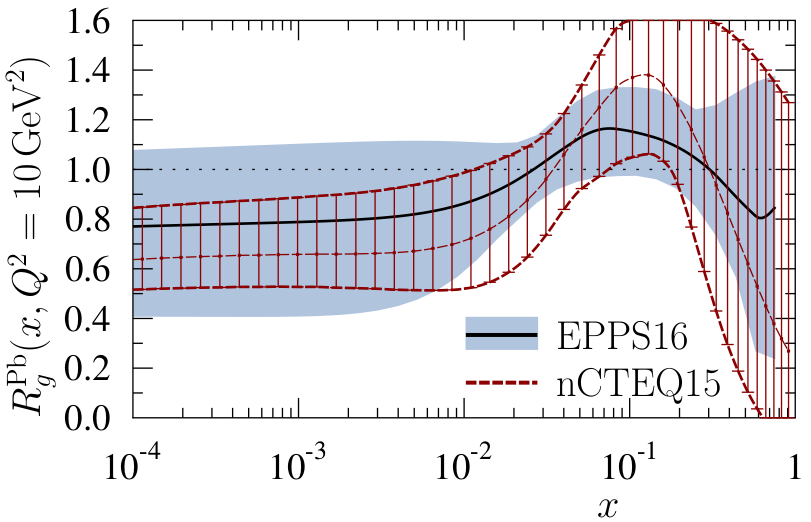
\includegraphics[width=0.7\textwidth]{Figures/Charmonia/Theory/HeavyIons/GluonNPDF.png}
 \caption{Gluon nuclear PDF modification factor determined with EPPS16 (black curve with blue band) and nCTEQ15 (red curves with hatching) nPDF calculations at $Q^{2} =\SI{10}{\square\GeV}$. Figure taken from Ref.~\cite{EPPS16}.}
 \label{fig:GluonNPDF}
\end{figure}

\paragraph{Energy loss and Cronin effect.} When high-energy partons traverse the nuclear medium, they lose energy through gluon radiation induced by multiple scatterings in the target nucleus, before or after the hard interaction. It has been proposed by Arleo \textit{et al.}~\cite{EnergyLoss_1,EnergyLoss_2,EnergyLoss_3}, that if the formation length of the radiated gluon is much larger than the size of the nucleus, the gluon radiation becomes coherent (i.e. the radiated gluon would see the nucleus as a whole). The coherent energy loss is proportional to the energy of the incident particle and it effectively decreases the rapidity of the hard particle.

Moreover, as high-energy partons undergo elastic scatterings in the nucleus, they gain transverse momentum in the process. As a consequence, the average partonic $\langle{\pt^{2}}\rangle$ (known as \pt-broadening) increases proportionally to the number of scattering centres encountered in the medium. These leads to an enhancement of the particle yields at intermediate \pt ($< 10$~\GeVc). This effect was discovered in 1974 by Cronin \textit{et al.}, in proton-tungsten collisions~\cite{CroninEffect}, and it is known as the Cronin effect.

The ALICE collaboration has measured the nuclear modification factor of \JPsi mesons in \RunpPb collisions at $\sqrtsnn = \SI{5.02}{\TeV}$~\cite{ALICE_JPsi_RAA_pPb_5p02TeV}. The results are shown in \fig{fig:EnergyLossALICE} as a function of \pt and compared to theory calculations including energy loss with (light green band) and without (dark green band) EPS09 nuclear PDFs. The theory calculations considering energy loss and gluon shadowing are found to be consistent with the measurements at $\pt > 2$~\GeVc, while those with only energy loss effects overestimate the results in the central and forward rapidity regions. Regarding the low \pt and forward region, the theory calculations expect a larger suppression of \JPsi mesons than what is observed in the measurements.

\begin{figure}[!htb]
 \centering
 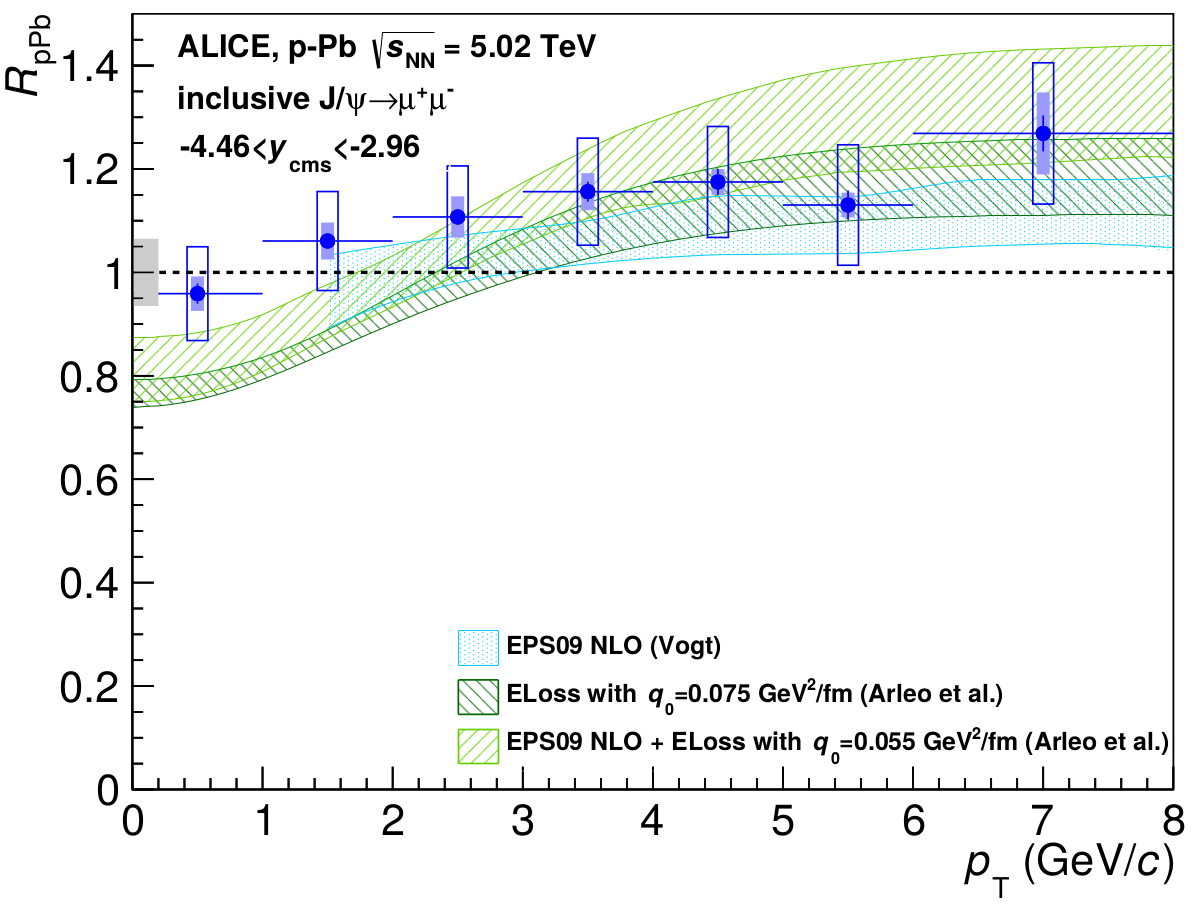
\includegraphics[width=0.45\textwidth]{Figures/Charmonia/Theory/HeavyIons/EnergyLossALICE_1.png}
 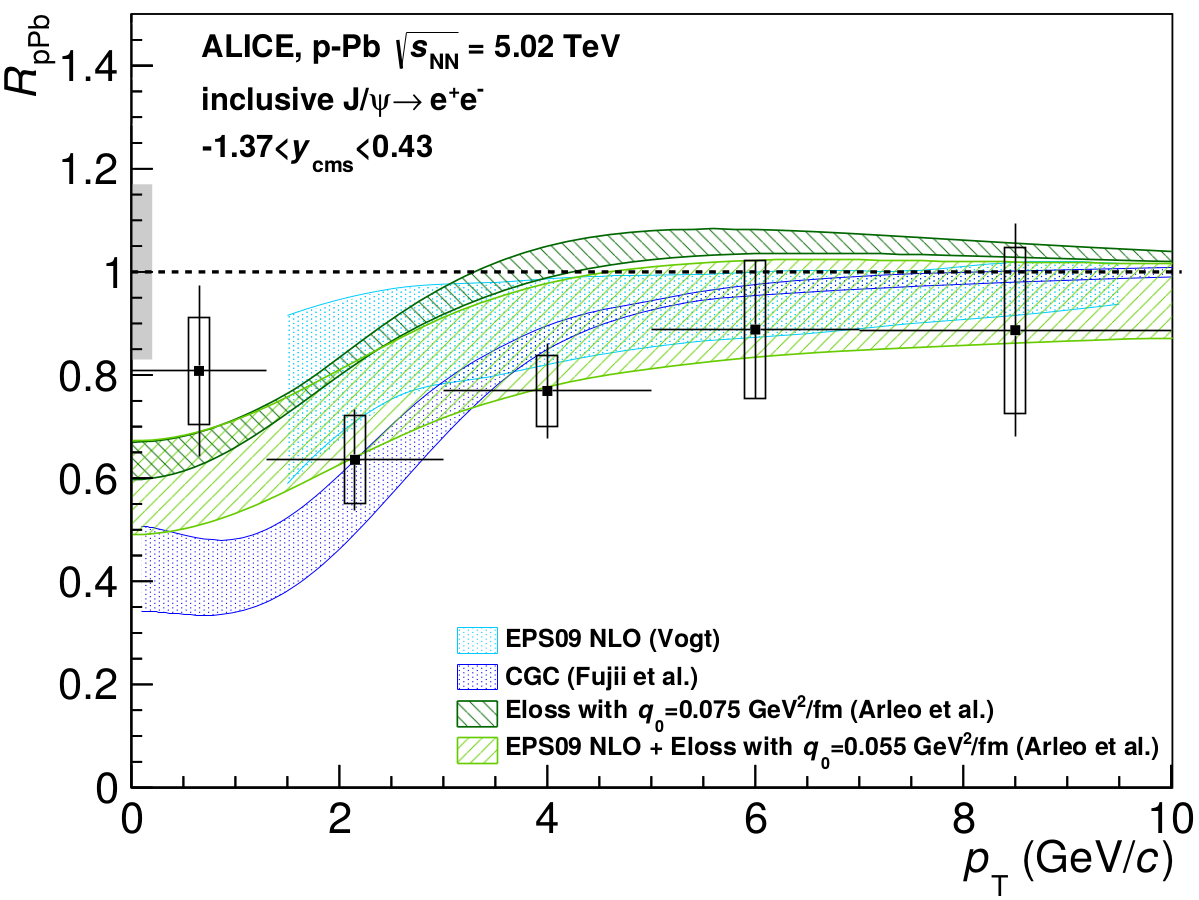
\includegraphics[width=0.45\textwidth]{Figures/Charmonia/Theory/HeavyIons/EnergyLossALICE_2.png}
 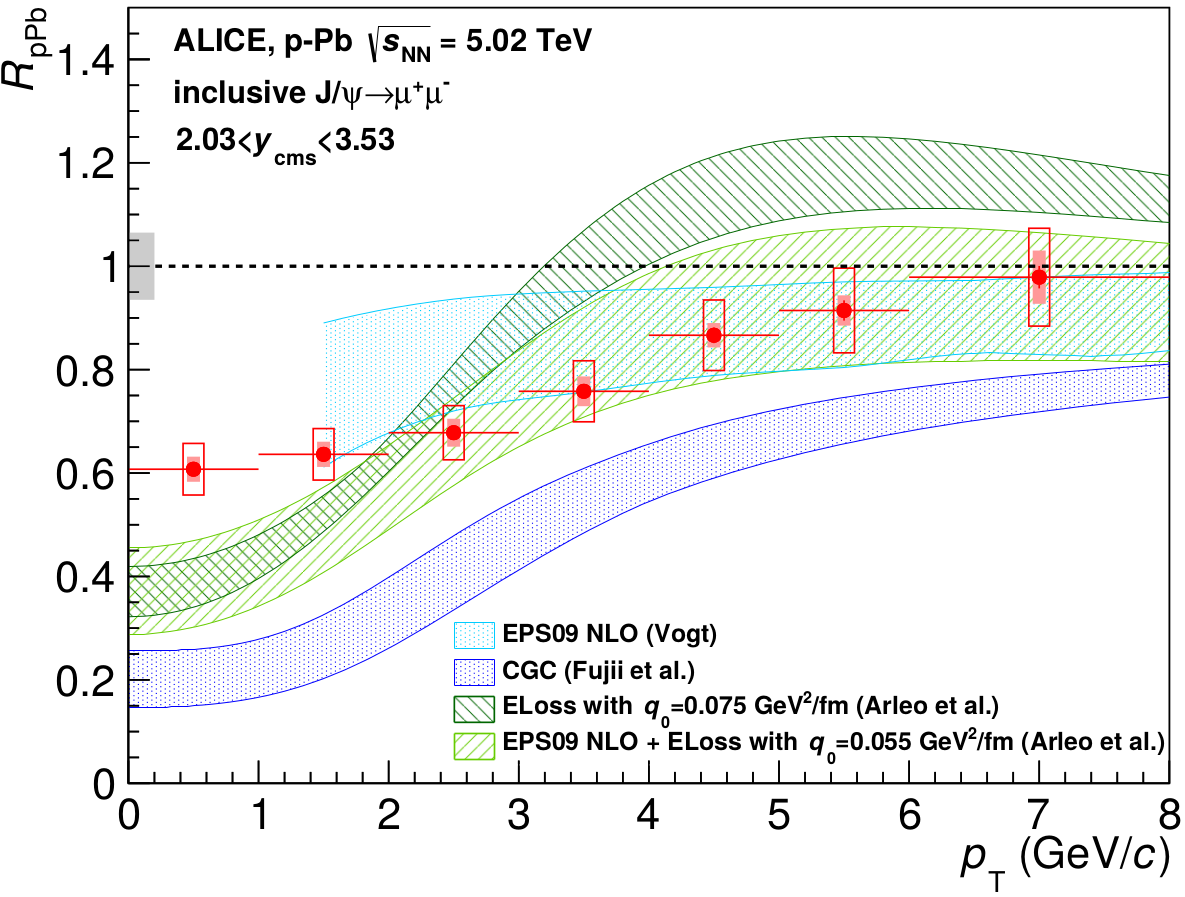
\includegraphics[width=0.45\textwidth]{Figures/Charmonia/Theory/HeavyIons/EnergyLossALICE_3.png}
 \caption{Nuclear modification factor of \JPsi mesons as a function of \pt in the backward (top-left), mid (top-right) and forward (bottom) rapidity regions. The bars (boxes) represent the statistical (systematic) uncertainties, while the gray box at unity indicate the size of the global uncertainty. The results are compared to nPDF (EPS09), energy loss (Arleo et al), and gluon saturation (CGC) calculations. Figure taken from Ref.~\cite{ALICE_JPsi_RAA_pPb_5p02TeV}.}
 \label{fig:EnergyLossALICE}
\end{figure}

\subsubsection{Hot nuclear matter effects}\label{sec:Charmonia_Theory_HeavyIon_HotNuclearMatter}

Charmonia are considered important probes of the QGP since they are produced in the initial hard scattering and experience the full evolution of the medium. The presence of the deconfined medium is expected to dissociate the charmonium states through a process called colour-charge screening, which can occur sequentially depending on the medium temperature and the charmonium binding energies. In addition, the large abundance of charm quarks at the LHC can lead to a recombination of uncorrelated charm quarks, enhancing the charmonium yields.

\paragraph{Colour-charge screening.} In the presence of the QGP, the binding potential of charmonia is screened by the colour charges of the surrounding quarks in the medium. This mechanism was first proposed in 1986 by Matsui and Satz~\cite{JpsiSuppression}. The colour-charge screening is described through a Debye screening radius $r_{D}\left(T\right) \propto 1/T$, which decreases for larger temperatures $T$ of the medium. If the Debye screening radius becomes smaller than the radius of a given charmonium state, the charm quarks are no longer able to maintain the bound state and the \ccbar pair dissociates. The \ccbar binding potential $V_{\ccbar}$, including the colour-charge screening effect, can be expressed as:

\begin{equation}
  V_{\ccbar}\left(r, T\right) = -\frac{a}{r}\exp\left[\frac{-r}{r_{D}\left(T\right)}\right] + b{\cdot}r_{D}\left(T\right)\left(1-\exp\left[\frac{-r}{r_{D}\left(T\right)}\right]\right)
\end{equation}

where if $r_{D} \rightarrow \infty$ (i.e. no screening, $T = 0$), one recovers the Cornell potential shown in \eq{eq:QQbar}. On the other hand, if $r_{D} \rightarrow 0$, the \ccbar binding potential becomes zero and the charm quarks are no longer confined. At the hadronisation stage, the deconfined charm quarks predominantly bound with light quarks, forming open-charm mesons and reducing the charmonium yields in the process.

Since the charmonium radius increases for higher excited states, as shown in \tab{tab:CharmoniumBindingEnergy}, it is expected that \PsiP mesons will dissociate at lower medium temperatures compared to \JPsi mesons, leading to a sequential suppression pattern. These effect can be quantified by comparing the nuclear modification factor of \PsiP mesons to the one of \JPsi mesons.

\begin{table}[htb!]
 \centering
 \begin{tabular}{| c | c | c |}
  \hline
  Charmonium state & Binding energy [\si{\GeV}] & Radius [fm] \\ \hline
  \JPsi & 0.64 & 0.25 \\ \hline
  $\chi_{\cPqc}(1\text{P})$ & 0.20 & 0.36 \\ \hline
  \PsiP & 0.05 & 0.45 \\
  \hline
 \end{tabular}
 \caption{Binding energy and radius of \JPsi, $\chi_{\cPqc}(1\text{P})$ and \PsiP mesons. Information taken from Ref.~\cite{Quarkonium_Overview}.}
 \label{tab:CharmoniumBindingEnergy}
\end{table}

\paragraph{Charmonium regeneration.} The charm-quark total cross section is large at the LHC, leading to an abundant production of charm and anti-charm quarks (up to 200 \ccbar pairs in a central \RunPbPb collision~\cite{UncorrelatedCharms_2}), which may combine to produce charmonium states. This additional source of charmonium production is expected to enhance the nuclear modification factor of charmonia. Since the thermal production of charm quarks (i.e. produced in the medium) is negligible, due to their large mass, the recombined \ccbar pairs are mainly formed by charm quarks produced in the hard scattering. This recombination mechanism, commonly known as charmonium regeneration, can be described using a statistical model~\cite{StatisticalHadronisation_1,JpsiRegeneration}, where the charm quarks are recombined during the hadronisation stage. Alternatively, the regeneration of charmonia can also be described using transport models~\cite{TransportModel_1}, where the charmonium states are continuously dissociating and regenerating throughout the evolution of the QGP. Since the uncorrelated charm quarks are required to be close in phase space, to be able to form a charmonium state, the regeneration mechanism mainly plays a role at low charmonium \pt and narrow rapidities.


\subsubsection{Current understanding}\label{sec:Charmonia_Theory_HeavyIon_CurrentStatus}

The suppression and regeneration of quarkonia, as a possible signature of the QGP, were briefly discussed in \sect{sec:Physics_HI_Probes_Quarkonium}. As was mentioned there, an anomalous suppression of \JPsi and \PsiP mesons in central collisions was already observed at SPS at $\sqrtsnn = \SI{17.3}{\GeV}$~\cite{SPSJpsiSuppression_1,SPSPsiPSuppression}, which could not be explained considering only CNM effects. Later, measurements performed at RHIC at $\sqrtsnn = \SI{200}{\GeV}$~\cite{JpsiRHIC} showed similar levels of \JPsi-meson suppression at mid-rapidity and stronger suppression at forward rapidity. Two explanations were proposed to describe the results at RHIC: the first one suggested that contributions from regenerated \JPsi mesons could accommodate the agreement observed between RHIC and SPS, while the second one was able to describe the differences seen between forward and mid-rapidity taking into account nPDF effects and nuclear absorption.

The production of \JPsi mesons has been measured at the LHC in \RunPbPb collisions at $\sqrtsnn = \SI{2.76}{\TeV}$. The general feature observed among the different LHC experiments is a strong suppression of charmonia ($\raa << 1$) in central collisions consistent with colour-charge screening. In addition, the ALICE collaboration has reported a weaker suppression of \JPsi mesons in particular at low \pt compared to RHIC measurements~\cite{ALICEJpsiRegeneration}, which has been attributed to \JPsi-meson regeneration. Measurements in \RunpPb collisions have also been performed at the LHC, which are found to be consistent with calculations including nuclear modifications of the PDFs and/or energy loss. However, the exact contributions of the various hot and cold nuclear matter effects are difficult to asses, specially due to the large uncertainties on the gluon nuclear PDFs and the limited statistical precision of the data. As a result, more precise and differential measurements are needed, both to constrain the models and to disentangle the different contributions that play a role in heavy-ion collisions.

As for bottomonia, measuring the excited states could bring important information. The CMS collaboration has reported the nuclear modification of \PsiP mesons relative to \JPsi mesons in \RunPbPb collisions at $\sqrtsnn = \SI{2.76}{\TeV}$~\cite{CMS_Psi2S_PbPb_2p76TeV}. The results of the double ratio of \PsiP over \JPsi yields, \doubleRatio, are presented as a function of \avgnpart in \fig{fig:DoubleRatio_CMS2p76}. The \PsiP mesons are observed to be more suppressed than \JPsi mesons at high \pt ($> 6.5$~\GeVc) in the mid-rapidity region, consistent with the sequential suppression scenario. On the contrary, in the forward rapidity region and moderate \pt range ($3 < \pt < 30$~\GeVc), the \PsiP mesons are found to be less suppressed than \JPsi mesons in the most central \RunPbPb collisions, which was unexpected at the time and still not fully understood. However, a similar measurement performed by the ALICE collaboration in central \RunPbPb collisions~\cite{ALICE_Charmonium_PbPb_2p76TeV}, extending down to $\pt = 0$~\GeVc, points to a larger \PsiP-meson suppression than for \JPsi mesons. Transport model calculations~\cite{DoubleRatioTheory} have attempted to explain the results by arguing that \PsiP and \JPsi mesons are regenerated at different stages of the QGP evolution, leading to possible weaker overall suppression of \PsiP relative to \JPsi mesons, depending on the region of phase space they probe.

\begin{figure}[!htb]
 \centering
 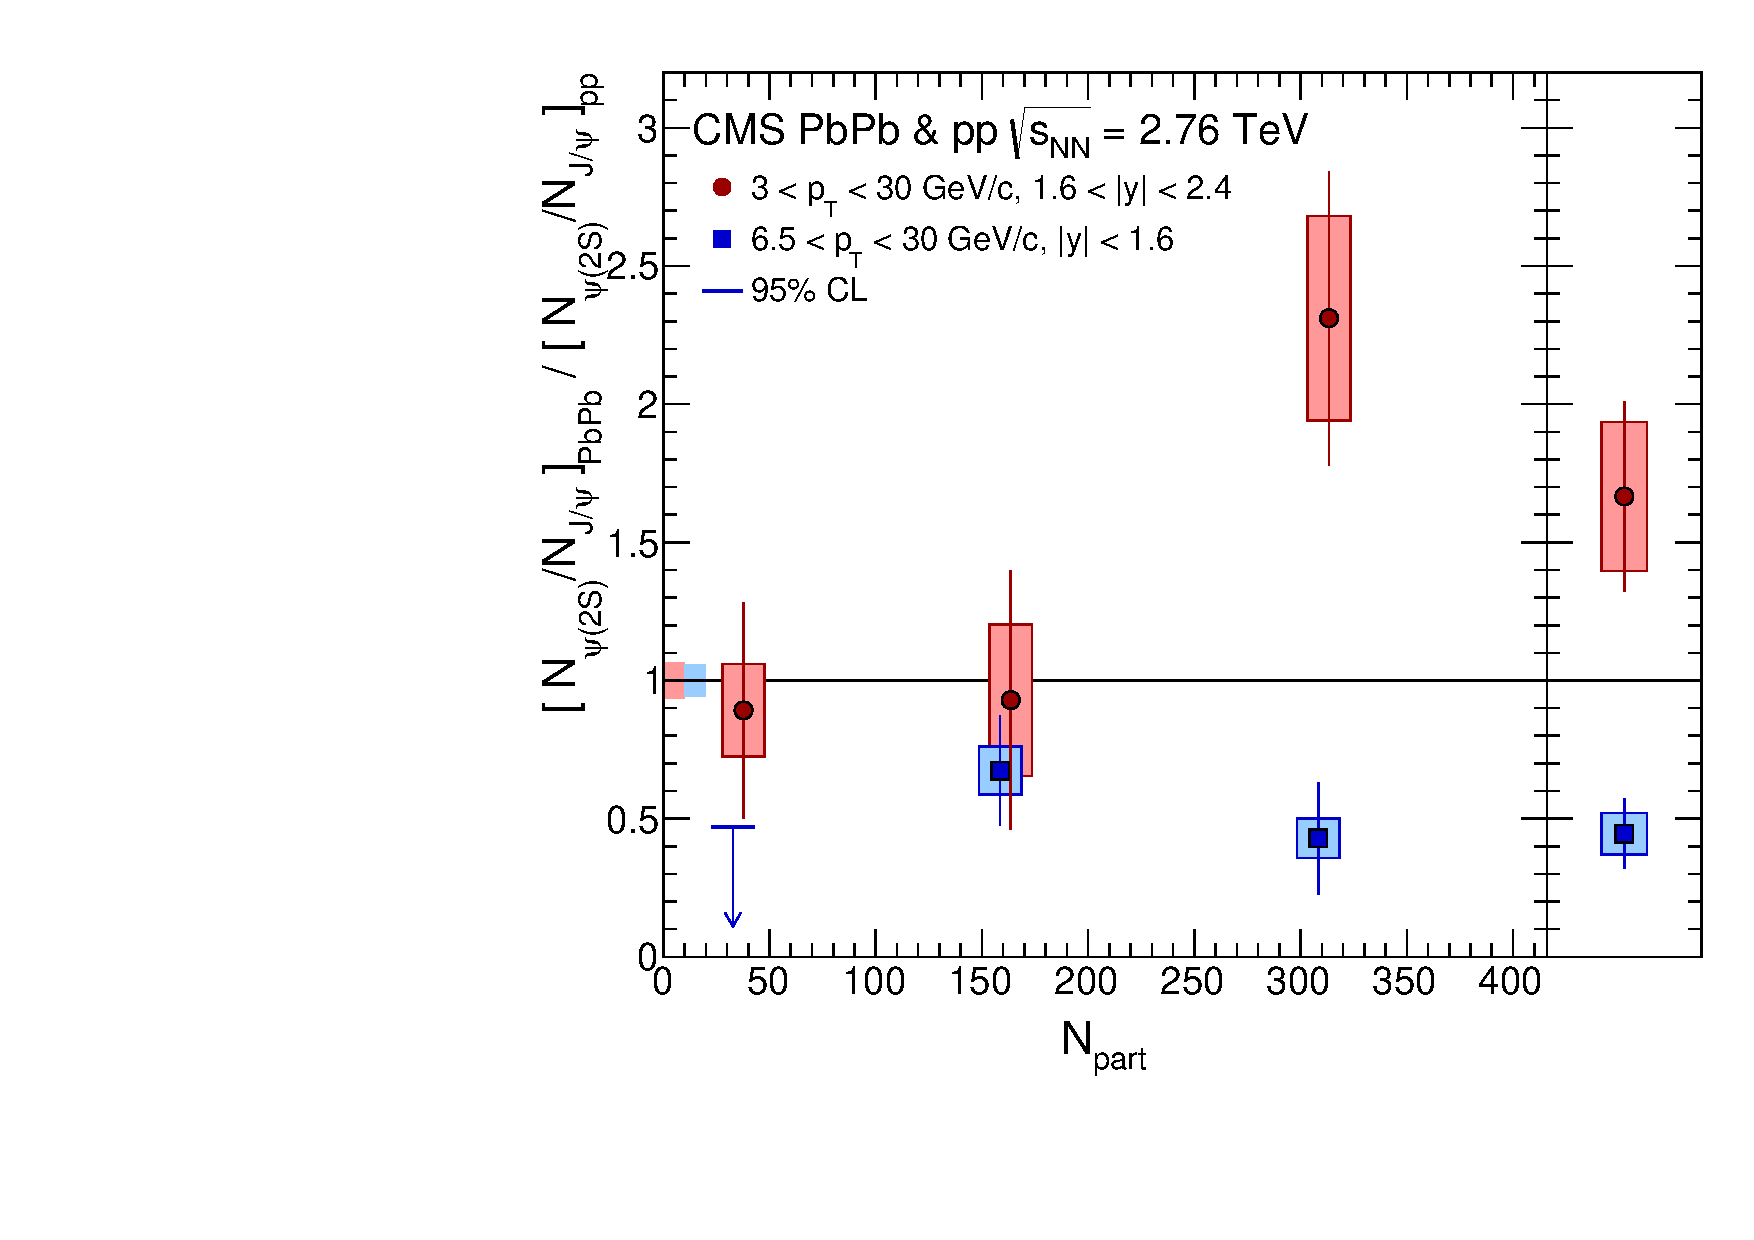
\includegraphics[width=0.6\textwidth]{Figures/Charmonia/Theory/HeavyIons/double_ratio.pdf}
 \caption{Double ratio of \PsiP over \JPsi yields as a function of \avgnpart, in the mid-rapidity (blue squares) and forward rapidity (red circles) regions. The results integrated in centrality are shown at the rightmost edge. The bars (boxes) represents the statistical (systematic) uncertainties, while the boxes at unity indicate the uncertainties on the \Runpp measurements. Figure taken from Ref.~\cite{CMS_Psi2S_PbPb_2p76TeV}.}
 \label{fig:DoubleRatio_CMS2p76}
\end{figure}

The measurements of the charmonium production in \RunPbPb collisions at $\sqrtsnn = \SI{5.02}{\TeV}$, presented in the following sections, benefits from a larger integrated luminosity ($\times 2$) and higher energy compared to the \RunPbPb measurements at $\sqrtsnn = \SI{2.76}{\TeV}$. This allows to extend the \pt reach of the measurements, increase the precision of the results and perform more differential studies.

% END OF SECTION